\documentclass[conference]{IEEEtran}
\IEEEoverridecommandlockouts
% The preceding line is only needed to identify funding in the first footnote. If that is unneeded, please comment it out.
\usepackage{cite}
\usepackage{amsmath,amssymb,amsfonts}
\usepackage{algorithmic}
\usepackage{graphicx}
\usepackage{textcomp}

\newcommand*{\Comb}[2]{{}_{#1}C_{#2}}%

\usepackage{tabularx,ragged2e}
\newcolumntype{C}{>{\Centering\arraybackslash}X} % centered "X" column
% \newcolumntype{b}{X}
\newcolumntype{s}{>{\hsize=.5\hsize}X}

\usepackage{xcolor}
\def\BibTeX{{\rm B\kern-.05em{\sc i\kern-.025em b}\kern-.08em
    T\kern-.1667em\lower.7ex\hbox{E}\kern-.125emX}}
\begin{document}

\title{Primi Composti: a Tabletop Game Analysis}

\author{
\IEEEauthorblockN{1\textsuperscript{st} Lorenzo Serafini}
\IEEEauthorblockA{
\textit{University Of Padua}\\
Padua, Italy \\
lorenzo.serafini.1@studenti.unipd.it}
\and
\IEEEauthorblockN{2\textsuperscript{nd} Michele Sprocatti}
\IEEEauthorblockA{
\textit{University Of Padua}\\
Padua, Italy \\
michele.sprocatti@studenti.unipd.it \\ https://orcid.org/0009-0005-7886-441X}
\and
\IEEEauthorblockN{3\textsuperscript{rd} Riccardo Zuech}
\IEEEauthorblockA{
\textit{University Of Padua}\\
Padua, Italy \\
riccardo.zuech@studenti.unipd.it}
}
\maketitle

\begin{abstract}
	This project has the objective of providing a game theoretic analysis of a real-world scenario, that is the tabletop game Primi Composti. In particular, we are interested into checking whether there is an inherent advantage into going first or second by considering all combinations of different practical strategies from a set we define.
	This project tackles some of the challenges that arise when applying game theoretic tools to real-world practical scenarios, like dealing with the random assignments of cards to the players and the high computational costs of standard best-response strategies.
	% This project aims at finding if the two players can have advantages by starting or by being the second player in the game of Primes Compounds. To test if this is true or not, we defined some well-known strategies, and we simulated the game for different assignments of initial cards for the different pairs of strategies that the two players can play. Then we have done some analysis on the results to see if there are some advantages, and in case this is true, understand also for which player or for which pair of strategies.
\end{abstract}

%\begin{IEEEkeywords}
%\end{IEEEkeywords}

\section{Motivation}
% Riccardo
\section{Strategies}
% Lorenzo
\section{Simulation} \label{section:Simulation} %Michele
In this section, we are going to refer to player 1 as P1 and player 2 as P2 for simplicity.

In order to understand if there is an inherit advantage into going first or second, we run several simulations and compare the outcomes of the games under all the combinations of two strategies from the ones explained in section \ref{section: Strategies}. Then, we consider two cases:
\begin{itemize}
    \item General case: whoever starts between P1 and P2 is decided by which player has the card 2 in its hand.
    \item P1 always starts: player P1 always gets the hand containing the 2, thus playing first.
\end{itemize}
To achieve our objective, we first generate $n$ pairs of random hands, one for each player. Then for each pair of hands, we simulate the game on every possible combination of two strategies from Section \ref{section: Strategies}. The simulation is run by supposing that each player sticks to his strategy for all possible situations that is a bit unrealistic because human players can change and adapt based on the opponent's moves, but for the sake of simplicity for the simulation, we made this assumption.

\subsection{Results} \label{subsection:Results}
To have enough data to make statistical analyses but also to have limited computation time, we decided to do $n = 10000$ samples of possible assignments; then we simulate the different strategies.

By looking at figure \ref{fig:comparison_pl1}, that plots the win of player 1 when the two players play the same strategy, we can see that there is some small advantage for some strategies (random, max, min, prime, comp, max\_val) versus a great worsening for two particular strategies (security, minimax).

This is also reflected in the opposite plot, so the one for player 2 reported in figure \ref{fig:comparison_pl2}.

\begin{figure}
    \centering
    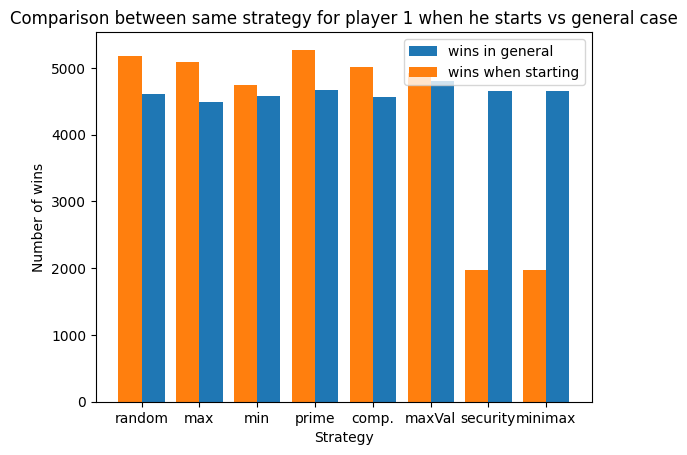
\includegraphics[width=1\linewidth]{img/comparison_winning_starts_general_pl1.png}
    \caption{Wins of player 1 in the two cases when the two players play the same strategy.}
    \label{fig:comparison_pl1}
\end{figure}

\begin{figure}
    \centering
    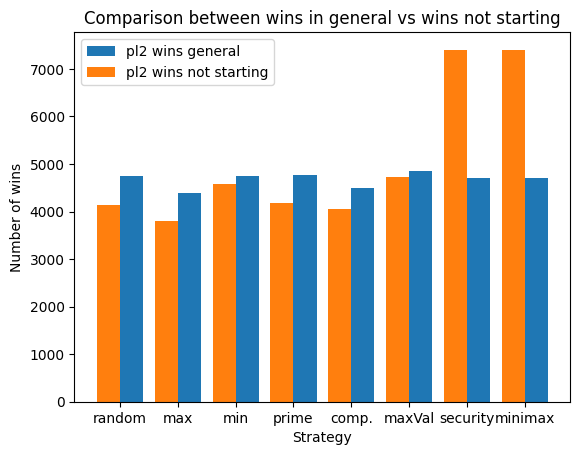
\includegraphics[width=1\linewidth]{img/comparison_winning_not_starts_general_pl2.png}
    \caption{Wins of player 2 in the two cases when the two players play the same strategy.}
    \label{fig:comparison_pl2}
\end{figure}

After these, we have computed the probability that player 1 wins the game for every possible pair of strategies. The probability is computed as follows:

\begin{equation} \label{eq:probability_cal}
    prob = \frac{number-of-wins}{number-of-total-matches}
\end{equation}

To visualize the results in these two cases, we decided to use the heat-maps; the plots are reported in figure \ref{fig:prob_general} and in figure \ref{fig:prob_starts}. 

From the plot in figure \ref{fig:prob_general} we can see that in the general case the probability of winning for player 1 and player 2 for the top-right is close to 50/50; but the chances that player 1 wins are very high when these combinations arise:
\begin{enumerate}
    \item max\_val vs random
    \item security vs random
    \item minimax vs random
    \item max\_val vs min
    \item security vs min
    \item minimax vs min
    \item security vs prime first
    \item minimax vs prime first
\end{enumerate}
The first 3 were somehow obvious because the second player is choosing the card randomly without a strategy, so a good strategy for player 1 will very likely beat player 2. The other five results instead are more interesting. 
Since the probability of winning for player 2 is $1 - probability-winning-player-1$ we can see the dark part at the top right of the heat-map.

By looking at figure \ref{fig:prob_starts} we can see what we have pointed out before using figure \ref{fig:comparison_pl1} and \ref{fig:comparison_pl2} that is the fact that we have a significant drop in the chance of winning for the strategies in the bottom right part of the heat-map, but we have an increasing probability for all the other combinations.

To visualize in a better way this last observation we plot also the difference between the two sets of probabilities and we obtained the heat-map in \ref{fig:diff_prob}, using this plot we can see that we have a 5 \% increment in the top left but a 25 \% decrease in the bottom right. So given these values we can say that maybe the player that does not start has an advantage because in certain pairs of strategies the probability of the starting player increases by a small percentage but it decreases a lot for other strategies so the not-starting player has in general a greater chance to win.

\begin{figure}
    \centering
    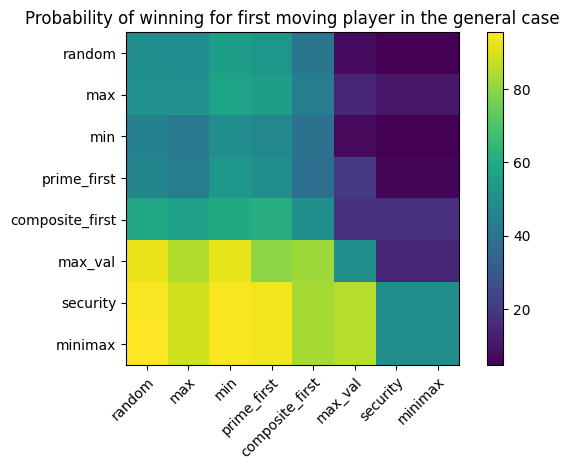
\includegraphics[width=1\linewidth]{img/prob_winning_general.png}
    \caption{Probability of winning for player 1 in general case (strategy of player 1 on the rows).}
    \label{fig:prob_general}
\end{figure}

\begin{figure}
    \centering
    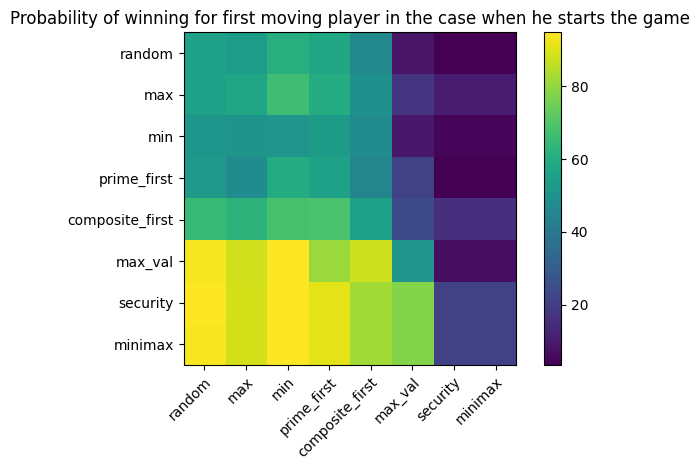
\includegraphics[width=1\linewidth]{img/prob_winning_starts.png}
    \caption{Probability of winning for player 1 in the case where he always starts (strategy of player 1 on the rows).}
    \label{fig:prob_starts}
\end{figure}

\begin{figure}
    \centering
    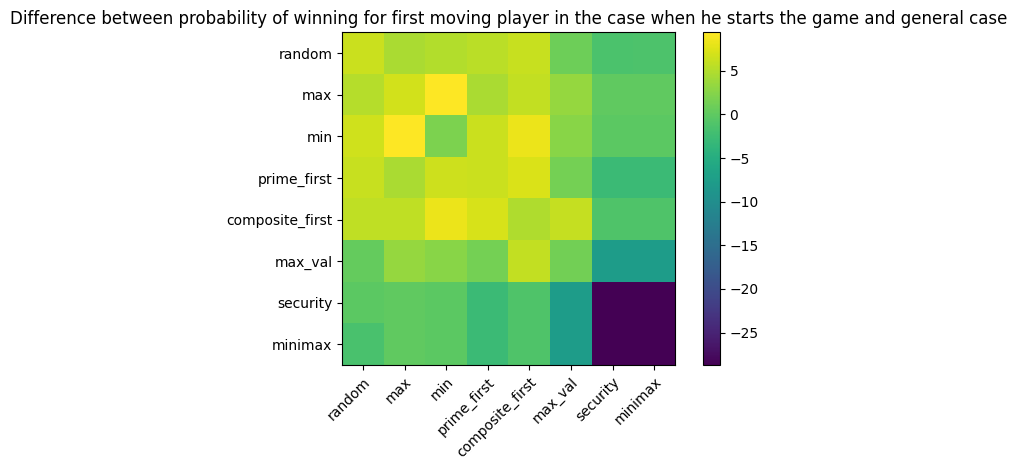
\includegraphics[width=1\linewidth]{img/diff_prob.png}
    \caption{Difference between probability of winning for player 1 when it starts and the general case.}
    \label{fig:diff_prob}
\end{figure}

For all possible simulations that we have run, we also collected the different scores of each match. These results are used in order to plot a box plot for each pair of strategies in the two cases that we have analyzed. These can be seen in figure \ref{fig:box_general} and figure \ref{fig:box_starts}.
From the comparison between these plots, we can see again the bottom left part where we have a worsening of the scores of player 1 from general to the case where it starts confirming again what we have said before. 
Also, we can see that, in general, we have very small boxes but very large whiskers; this means that we have a large variance of the scores but also that in the 2\textsuperscript{nd} and 3\textsuperscript{rd} quantiles we have data that is very concentrated. We can also see that there are a lot of outliers pretty much everywhere. In particular, we can see that when player 1 starts, the number of outliers increases a lot for both players.

\begin{figure}
    \centering
    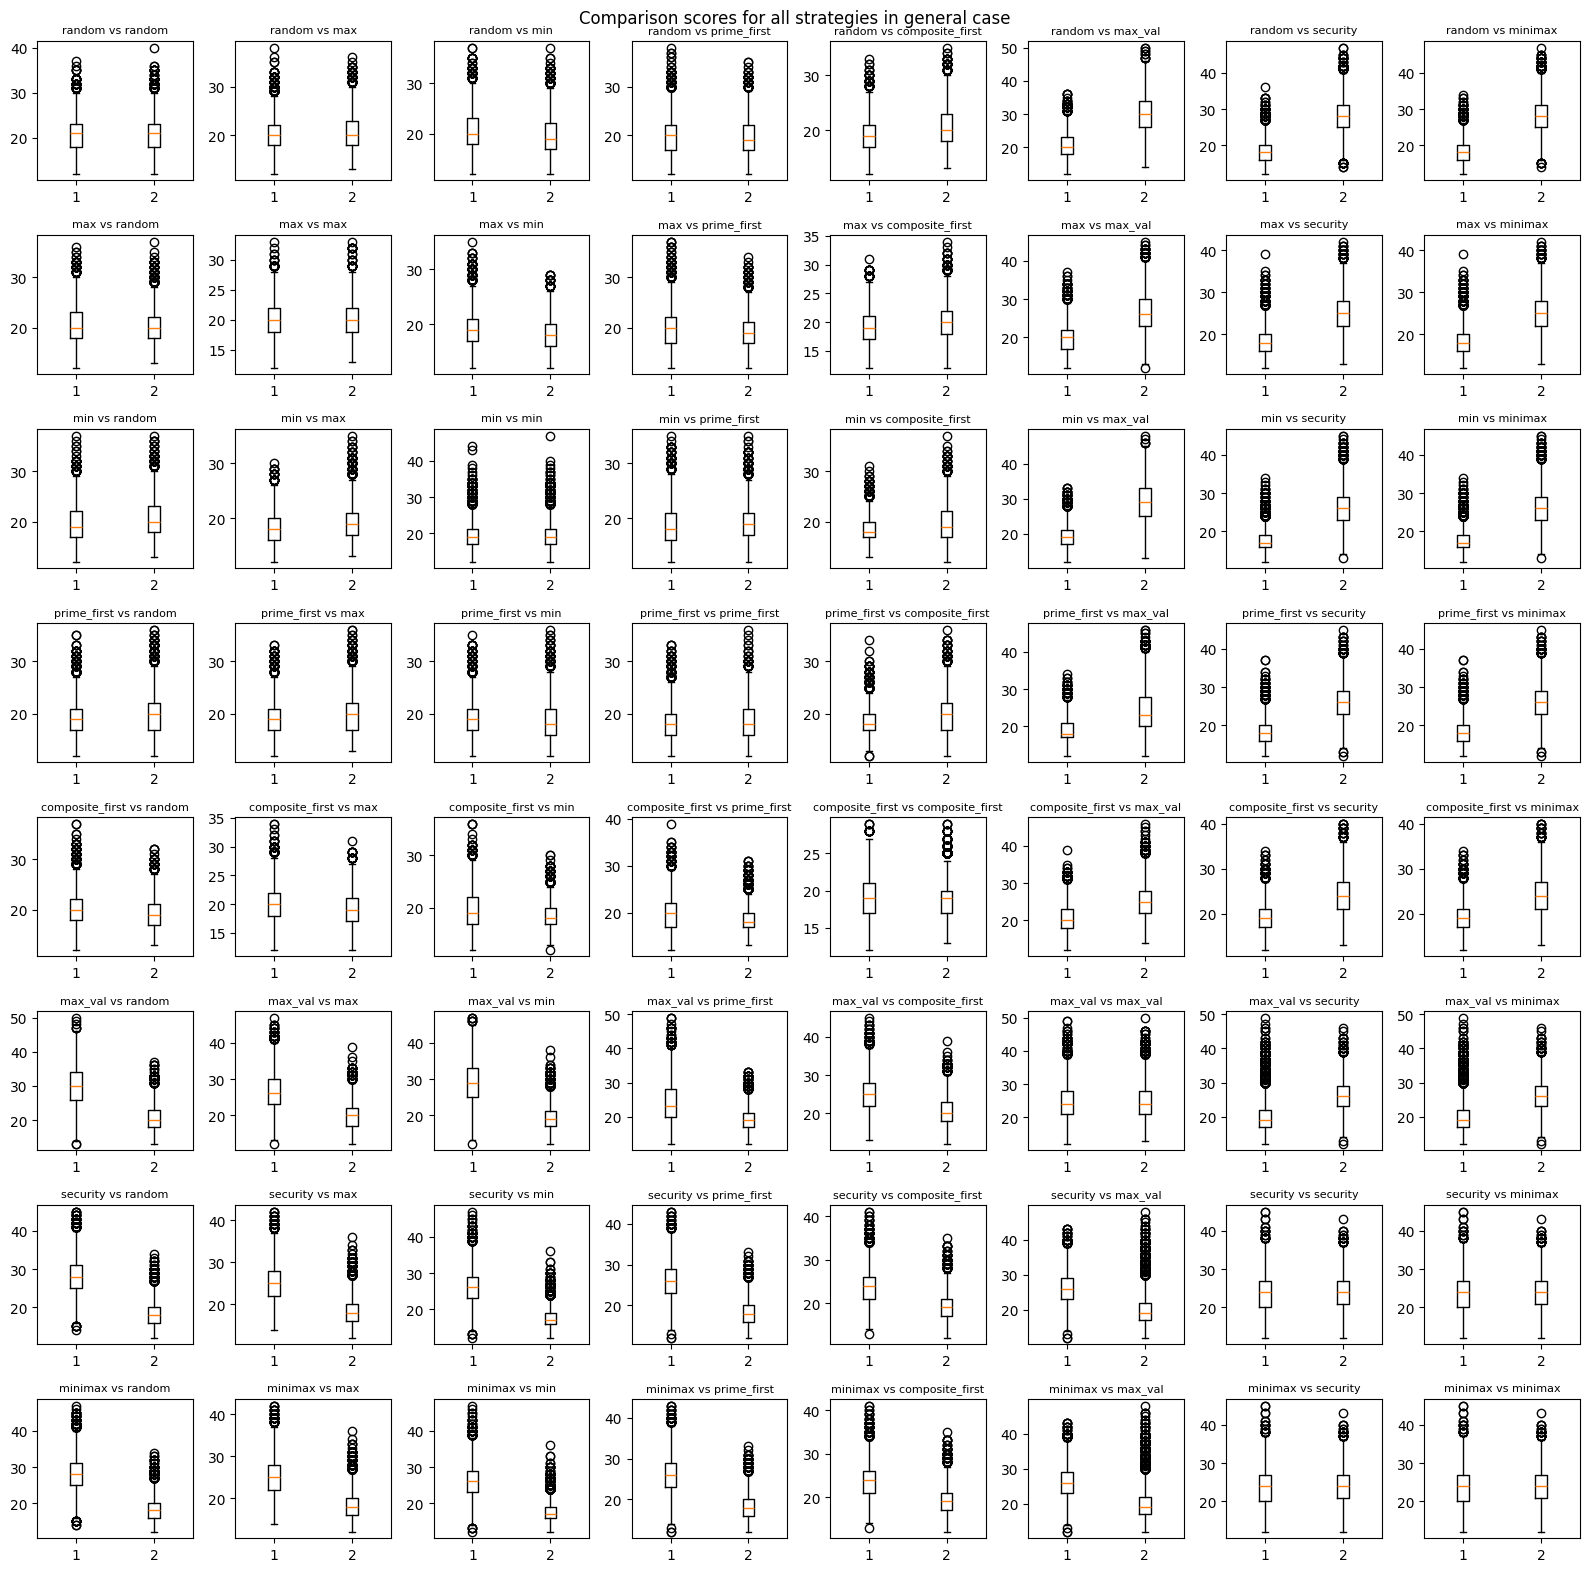
\includegraphics[width=1\linewidth]{img/box_plot_general.png}
    \caption{Plot that reports the box plots of the different score for each pair of strategies in the general case.}
    \label{fig:box_general}
\end{figure}

\begin{figure}
    \centering
    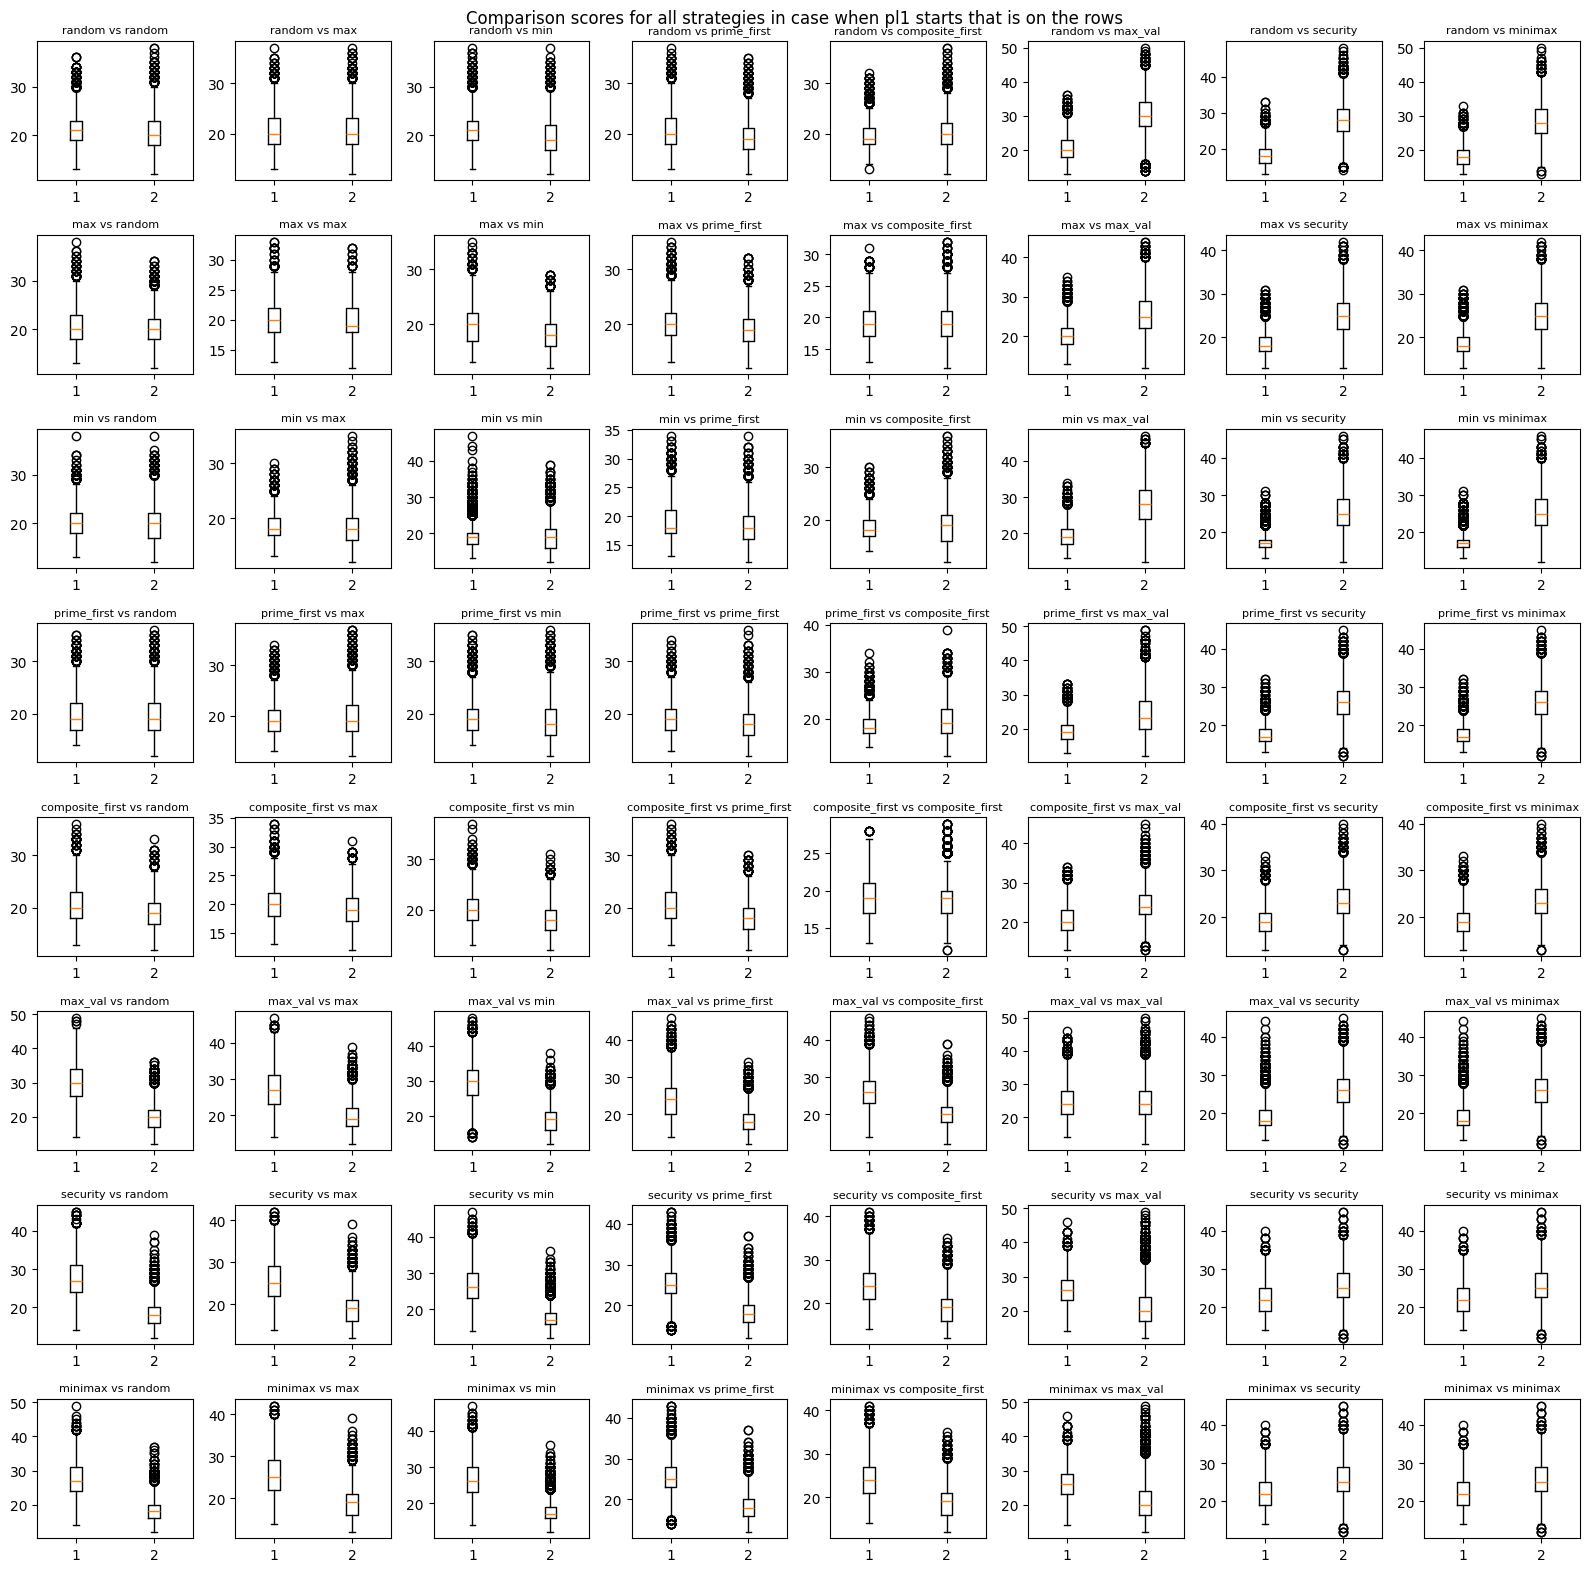
\includegraphics[width=1\linewidth]{img/box_plot_starts.png}
    \caption{Plot that reports the box plots of the different score for each pair of strategies when player 1 starts.}
    \label{fig:box_starts}
\end{figure}

At the end of the code, there is also a small part that uses an optimization method to find the binomial distribution that best fits the data in the two cases. The distributions found are very similar to the ones computed before using the equation \ref{eq:probability_cal}.
\section{Conclusions} \label{section:Conclusions} % Michele
Our analysis indicates that the game, in its general form, exhibits a balanced design. The observed winning probabilities for the majority of strategies converge towards a 50/50 distribution as you can see in figure \ref{fig:prob_general}, suggesting a fair game. While certain strategies deviate from this balance, leading to unbalanced probabilities, these instances are confined to a narrow subset of strategies that are less realistic.

To investigate potential first-mover or second-mover advantages, we analyzed the game dynamics with a fixed starting player. Our findings suggest that such advantages are negligible. The observed variations in winning probabilities when comparing the general case with the scenario where Player 1 always starts are minimal, with a modest 5 \% increase. Furthermore, there are some significant shifts in winning probability, 25 \% decrease for the starting player, but these decreases are primarily observed within the unrealistic strategies considered before. So we can say that we don't have first-mover or second-mover advantages.

\section*{Acknowledgment}


\section*{References}


\end{document}

